%latex model.tex
%bibtex model
%dvipdfm model.dvi

\documentclass[runningheads,a4paper,11pt]{report}
\usepackage{multicol}
\usepackage[table,xcdraw]{xcolor}
\usepackage{algorithmic}
\usepackage{algorithm} 
\usepackage{array}
\usepackage{amsmath}
\usepackage{amsfonts}
\usepackage{amssymb}
\usepackage{amsthm}
\usepackage{caption}
\usepackage{comment} 
\usepackage{epsfig} 
\usepackage{fancyhdr}
\usepackage[T1]{fontenc}
\usepackage{geometry} 
\usepackage{graphicx}
\usepackage[colorlinks]{hyperref} 
\usepackage[latin1]{inputenc}
\usepackage{multicol}
\usepackage{multirow} 
\usepackage{rotating}
\usepackage{setspace}
\usepackage{subfigure}
\usepackage{url}
\usepackage{verbatim}
\usepackage{xcolor}

\geometry{a4paper,top=3cm,left=2cm,right=2cm,bottom=3cm}

\pagestyle{fancy}
\fancyhf{}
\fancyhead[LE,RO]{Emotion Recognition}
\fancyhead[RE,LO]{Alex \& Melania}
\fancyfoot[RE,LO]{ITSG 2019-2020}
\fancyfoot[LE,RO]{\thepage}

\renewcommand{\headrulewidth}{2pt}
\renewcommand{\footrulewidth}{1pt}
\renewcommand{\headrule}{\hbox to\headwidth{%
  \color{lime}\leaders\hrule height \headrulewidth\hfill}}
\renewcommand{\footrule}{\hbox to\headwidth{%
  \color{lime}\leaders\hrule height \footrulewidth\hfill}}

\hypersetup{
pdftitle={EmotionsReport},
pdfauthor={Alex&Melania},
pdfkeywords={pdf, latex, tex, ps2pdf, dvipdfm, pdflatex},
bookmarksnumbered,
pdfstartview={FitH},
urlcolor=cyan,
colorlinks=true,
linkcolor=red,
citecolor=green,
}
% \pagestyle{plain}

\setcounter{secnumdepth}{3}
\setcounter{tocdepth}{3}

\linespread{1}

% \pagestyle{myheadings}

\makeindex


\begin{document}

\begin{titlepage}
\sloppy
\begin{center}
BABE\c S BOLYAI UNIVERSITY, CLUJ NAPOCA, ROM\^ ANIA

FACULTY OF MATHEMATICS AND COMPUTER SCIENCE

\vspace{6cm}

\Huge \textbf{EMOTION RECOGNITION}

\vspace{1cm}

\normalsize -- ITSG report --

\end{center}


\vspace{5cm}

\begin{flushright}
\Large{\textbf{Team members}}\\
Bartha Melania Beata, SDI, 254\\
Pirvu Alexandru, SDI, 254
\end{flushright}

\vspace{4cm}

\begin{center}
2019
\end{center}

\end{titlepage}

\pagenumbering{gobble}

\begin{abstract}
	Text of abstract. Short info about: project relevance/importance, inteligent methods used for solving, data involved in the numerical experiments; conclude by the the results obtained.
\end{abstract}


\tableofcontents

\newpage

\listoftables
\listoffigures
\listofalgorithms

\newpage

\setstretch{1.5}



\newpage

\pagenumbering{arabic}


 


\chapter{Introduction}
\label{chapter:introduction}

\section{What? Why? How?}
\label{section:what}

We want an objective measurement of the emotions that children experience during the interaction. This requires the development of an application that allows the identification of the emotional states of a preschooler during the course of an activity. We need to associate tasks that children do and the frequency of an emotion.
We want to detect emotions through facial expressions. For this association we need artificial intelligence algorithms. 

We then use support vector machines to classify the facial expressions and emotions.
Support vector machines have been proven useful in a number of pattern recognition tasks including face and facial action recognition.

\section{Paper structure and original contribution(s)}
\label{section:structure}

The research presented in this paper advances the theory, design, and implementation of several particular models. 

The main contribution of this report is to present an intelligent algorithm for solving the problem of $\ldots$.

The second contribution of this report consists of building an intuitive, easy-to-use and user
friendly software application. Our aim is to build an algorithm that will help $\ldots$.

The third contribution of this thesis consists of $\ldots$.


The present work contains $xyz$ bibliographical references and is structured in five chapters as follows.

The first chapter/section is a short introduction in $\ldots$.

The second chapter/section describes $\ldots$.

The chapter/section \ref{chapter:proposedApproach} details $\ldots$.



\chapter{Scientific Problem}
\label{section:scientificProblem}


\section{Problem definition}
\label{section:problemDefinition}

Give a description of the problem.
Explain why it must be solved by an intelligent algorithm. 
Details the advantages and/or disadvantages of solving the problem by a (some) given method(s).

Precisely define the problem you are addressing (i.e. formally specify the inputs and outputs). Elaborate on why this is an interesting and important problem.


Item example: 

\begin{itemize}
	\item content of item1
 	\item content of item2
 	\item content of item3
\end{itemize}



Figure example 

$\ldots$ (see Figure \ref{swarmsize})

\begin{figure}[htbp]
	\centerline{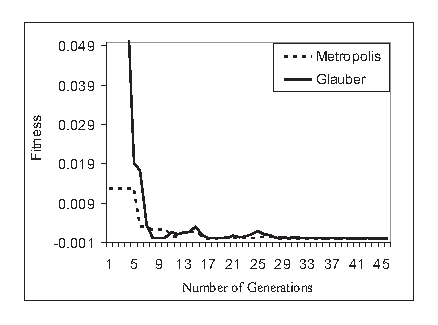
\includegraphics{Fig/FitEvol.eps}}  
	\caption{The evolution of the swarm size during the GA generations. This results were obtained for the $f_2$ test function with 5 dimensions.}
	\label{swarmsize}
\end{figure}


Table example: (see Table \ref{tab3PSO})


\begin{table}[htbp]
	\caption{The parameters of the PSO algorithm (the micro level algorithm) used to compute the fitness of a GA chromosome.}
	\label{tab3PSO}
		\begin{center}
			\begin{tabular}{p{220pt}c}

				\textbf{Parameter}& \textbf{Value} \\
				\hline\hline
 				Number of generations& 50 \\
 				Number of function evaluations/generation& 10 \\
 				Number of dimensions of the function to be optimized& 5 \\
 				Learning factor $c_{1}$& 2 \\
 				Learning factor $c_{2}$ & 1.8\\
 				Inertia weight& 0.5 + $\frac{rand()}{2}$\\
		
			\end{tabular}
		\end{center}
\end{table}

Algorithm example 

$\ldots$ (see Algorithm \ref{NGalg}).


\algsetup{indent=1em, linenosize=\footnotesize}

\begin{algorithm}
	\caption{SGA - Spin based Genetic AQlgorithm}
	\label{NGalg}
		\begin{algorithmic}


			\STATE \textbf{BEGIN}
  		\STATE @ Randomly create the initial GA population.
  		\STATE @ Compute the fitness of each individual.
  		\FOR{i=1 TO NoOfGenerations}
  			\FOR{j=1 TO PopulationSize}
  				\STATE p $\leftarrow$ RandomlySelectParticleFromGrid();
  				\STATE n $\leftarrow$ RandomlySelectParticleFromNeighbors(p);
  				\STATE @ Crossover(p, n, off);
  				\STATE @ Compute energy $\Delta H$
  				\IF {$\Delta H$ satisfy the Ising condition}
  					\STATE @ Replace(p,off);
  				\ENDIF
  			\ENDFOR
  		\ENDFOR
  		\STATE \textbf{END}
\end{algorithmic}
\end{algorithm}


\chapter{State of art/Related work}
\label{chapter:stateOfArt}

Automatically detecting facial expressions has become an increasingly important research area.

In 2000, the Cohn-Kanade database was released for the purpose of promoting research into automatically detecting individual facial expressions. \cite{Lucey10}
They recorded facial behavior of 210 adults. Participants were 18 to 50 years of age, 69\% female, 81\%, Euro-American, 13\% Afro-American, and 6\% other groups. For the CK+ distribution, they have augmented the dataset further to include 593 sequences from 123 subjects.
They identified 7 basic emotion categories: Anger, Contempt, Disgust, Fear, Happy, Sadness and Surprise.
They uses support vector machines to classify the facial expressions and emotions.

Their results were considerable and the hit rates for each emotion were : Angry - 75.00\%, Disgust - 94.74\%, Fear - 65.22\%, Happy - 100\%, Sadness - 68.00\%, Surprised - 77.09\%, Neutral - 100\%. \cite{Lucey10}


Tarnowski et. al in their article presented the results of recognition of seven emotional states. Coefficients describing elements of facial expressions, registered for six men aged 26-50, were used.
Each subject participated in two sessions. A participant mimicked all seven examined emotional states. As a result, 42 5-second sessions were registered for each user. The entire database contained a total of 252 facial expressions. \cite{Tarnowski17}
They used nearest neighbor classifier (3-NN) and two-layer neural network classifier (MLP) with 7 neurons in the hidden layer.
The input of the network were six AU, and the output was one of the seven emotional states.

They tested two ways to recognize emotions: a) subject-dependent - for each user separately and b) subject-independent - for all users together. In both cases, for 3-NN classifier, data were randomly divided on the teaching part (70\%) and the testing part (30\%) and for MLP into three groups: teaching (70\%), testing (15\%) and validation (15\%).
In subject-independent approach, the classifier accuracies (CA) for 3-NN and MLP algorithms were respectively 95.5\% and 75.9\%.
For user-independent classification the highest classification accuracy (73\%) was achieved for MLP neural network. \cite{Tarnowski17}




\chapter{Proposed approach}
\label{chapter:proposedApproach}

Useful tools: 
\begin{itemize}
\item OpenCV (Open source computer vision) is a library of programming functions mainly aimed at real-time computer vision. With OpenCV we can detect landmarks of all the faces found in an image and use them further in emotion detection.
\item Scikit-learn is a software machine learning library for Python. It features various classification, regression and clustering algorithms including support vector machines, random forests, gradient boosting, k-means and DBSCAN.
\end{itemize}

\textbf{Open Face}
Facial Action Coding System (FACS) is a system to taxonomize human facial movements by their appearance on the face. Movements of individual facial muscles are encoded by FACS from slight different instant changes in facial appearance. Using FACS it is possible to code nearly any anatomically possible facial expression, deconstructing it into the specific Action Units (AU) that produced the expression. It is a common standard to objectively describe facial expressions.

OpenFace is able to recognize a subset of AUs, specifically: 1, 2, 4, 5, 6, 7, 9, 10, 12, 14, 15, 17, 20, 23, 25, 26, 28, and 45. \cite{Baltrusaitis18}

\include{tableAU}

\textbf{
\section{Dataset}
}
We used for training the the Extended Cohn-Kanade Dataset (CK+).
Facial behavior of 210 adults was recorded using two
hardware synchronized Panasonic AG-7500 cameras. Participants
were 18 to 50 years of age, 69\% female, 81\%,
Euro-American, 13\% Afro-American, and 6\% other groups.
Image sequences for frontal views and 30-degree views were
digitized into either 640x490 or 640x480 pixel arrays with
8- bit gray-scale or 24-bit color values. Full details of this
database are given in.
For the CK+ distribution, they have augmented the dataset further to include 593 sequences from 123 subjects  The image sequence vary
in duration (i.e. 10 to 60 frames) and incorporate the onset
(which is also the neutral frame) to peak formation of the
facial expressions.
In this Phase there are 4 zipped up files. They relate to:

1) The Images -  there are 593 sequences across 123 subjects which are FACS coded at the peak frame. All sequences are from the neutral face to the peak expression.
2) The Landmarks - All sequences are AAM tracked with 68points landmarks for each image. 
3) The FACS coded files - for each sequence (593) there is only 1 FACS file, which is the last frame (the peak frame). Each line of the file corresponds to a specific AU and then the intensity. An example is given below.
4) The Emotion coded files  - ONLY 327 of the 593 sequences have emotion sequences. This is because these are the only ones the fit the prototypic definition. Like the FACS files, there is only 1 Emotion file for each sequence which is the last frame (the peak frame). There should be only one entry and the number will range from 0-7 (i.e. 0=neutral, 1=anger, 2=contempt, 3=disgust, 4=fear, 5=happy, 6=sadness, 7=surprise).\cite{Lucey10}

CAFE \cite{LoBue14}


\textbf{
\section{Training}
}
Scikit-learn is a software machine learning library for Python. It features various classification, regression and clustering algorithms including support vector machines, random forests, gradient boosting, k-means and DBSCAN.

\subsection{Support vector machines
}
Using Scikit-learn's support vector machines.

{
\section{Testing and Results}
}
For an image give the emotion \\
\includegraphics[width=6cm, height=5.5cm]{sad}
SADNESS\\



\chapter{Application (numerical validation)}
\label{chapter:application}


Explain the experimental methodology and the numerical results obtained with your approach and the state of art approache(s).

Try to perform a comparison of several approaches.

Statistical validation of the results.


\section{Methodology}
\label{section:methodology}

\begin{itemize}
	\item What are criteria you are using to evaluate your method? 
	\item What specific hypotheses does your experiment test? Describe the experimental methodology that you used. 
	\item What are the dependent and independent variables? 
	\item What is the training/test data that was used, and why is it realistic or interesting? Exactly what performance data did you collect and how are you presenting and analyzing it? Comparisons to competing methods that address the same problem are particularly useful.
\end{itemize}

\section{Data}
\label{section:data}

Describe the used data.

\section{Results}
\label{section:results}

Present the quantitative results of your experiments. Graphical data presentation such as graphs and histograms are frequently better than tables. What are the basic differences revealed in the data. Are they statistically significant?

\section{Discussion}
\label{section:discussion}

\begin{itemize}
	\item Is your hypothesis supported? 
	\item What conclusions do the results support about the strengths and weaknesses of your method compared to other methods? 
	\item How can the results be explained in terms of the underlying properties of the algorithm and/or the data. 
\end{itemize}



\chapter{Conclusion and future work}
\label{chapter:concl}

Try to emphasise the strengths and the weaknesses of your approach.
What are the major shortcomings of your current method? For each shortcoming, propose additions or enhancements that would help overcome it. 

Briefly summarize the important results and conclusions presented in the paper. 

\begin{itemize}
	\item What are the most important points illustrated by your work? 
	\item How will your results improve future research and applications in the area? 
\end{itemize}


\bibliographystyle{plain}
\bibliography{BibAll}

\end{document}
